\documentclass[preprint,NumberedRefs]{JASA}


\begin{document}

\title[Transverse-longitudinal reconstruction]{Reconstruction of transverse-longitudinal vibrations in the organ of Corti complex via optical coherence tomography}
\author{Brian L. Frost}
\affiliation{Department of Electrical Engineering, Columbia University, 500 W. 120th St., Mudd 1310, New York, NY 1002, USA.}
\email{b.frost@columbia.edu}
\author{Clark Elliott Strimbu}
\affiliation{Department of Otolaryngolgy Head and Neck Surgery, Vagelos College of Physicians and Surgeons, Columbia University, 630 W 168th St, New York, NY 10032.}
\author{Elizabeth S. Olson}
\affiliation{Department Biomedical Engineering, Columbia University, 351 Engineering Terrace, 1210 Amsterdam Avenue,New York, NY 10027. Also at Department of Otolaryngolgy Head and Neck Surgery.}

\preprint{Frost, JASA}

\date{\today} 


\begin{abstract}

\end{abstract}


\maketitle

\section{Introduction}
\par{Optical coherence tomography (OCT) is a powerful instrument for the study of cochlear mechanics. It is capable both of volumetric imaging and sub-nanometer vibrometry at a depth into a sample \citep{OCTtheory,sdpm}, allowing for the measurement of motion inside of the organ of Corti complex (OCC) \textit{in vivo} \citep{gao,dongoghalai,fallah,strimbu2020,fangyi,lee,cooper}. These data have provide significant insight into OCC micromechanics, both improving our understanding of and raising many questions about the mechanisms responsible for the incredible dynamic range of the sensitive cochlea. However, certain limitations of OCT can greatly complicate the interpretation of these data.}
\par{OCT vibration measurements and images are built from one-dimensional axial scans (A-Scans), generated via the Fourier transform of raw photodetector data. The magnitude of the A-Scan indicates the reflectivity at different depths into the sample. Images (referred to as brightness scans, or B-Scans) are built by taking a series of A-Scans along a line perpendicular to the optical axis. Many parallel B-Scans can be taken to form a volume scan.}
\par{A series of A-Scans at one location is referred to as a motion scan (M-Scan). The phase of a single pixel as a function of time is proportional to the sub-pixel displacement \textit{along the axis of the beam} of structures at that position \citep{sdpm}. That is, an M-Scan allows us to measure a projection of the 3-D motion of a structure onto the beam axis.}
\par{The nature of the modality leads to several important complications: (1) as OCT images are based on reflectivity, they are \textit{label-free}, so structures must be identified via known anatomy and intuition; (2) displacement measurements are 1-D projections of 3-D motions. These issues are even further complicated by the fact that the optical axis is often decided via the constraints of the preparation, and its relationship to the anatomy is often not known \textit{a priori}.}
\par{We have discussed these issues in terms of the anatomical coordinates of the cochlea (longitudinal, radial and transverse), using volume scans to determine the optical axis' relation to more physiologically relevant axes \citep{frost2022}. Using this method, one can account for the longitudinal (tonotopic) distance between measured points in a single A-Scan. One can also determine which components of motion are most represented in a measurement, offering more context to reported results. However, even this is not sufficient to separate out the motion components themselves.}
\par{It has been shown by Cooper et al that viewing angle can significantly impact both the magnitude and phase response of the structures being measured \citep{cooper2018}. Moreover, recent purely transverse measurements in the gerbil base have shown different character than measurements taken at an angle relative to basilar membrane (BM) normal \citep{Puria2022}. FOR EXAMPLE SEE FIG WHICH EXPLAINS DIFFERENCE BETWEEN TRANSV AND ANGLED MEAS}
\par{Several methods have been developed to attempt to address this problem. Lee et al used back-projection of measurements taken at two different angles to reconstruct radial-transverse motion in mouse, via carefully rotating the preparation to ensure they stay in the same cross-section \citep{lee}. Kim et al used a three-beam OCT system in mouse to measure motion at the same location from three angles, and back-project to resolve three-dimensional motion CITE. These methods are challenging to implement in the gerbil base, where the anatomy and opacity of the bone significantly restricts the beam angle when viewing through the round window (RW). The latter method also requires significant hardware and space.}
\par{We have developed a method to reconstruct the longitudinal and transverse components of motion \textit{in vivo} via OCT. Similar to the work described above, we reconstruct via back-projecting measurements taken at two angles. However, our method performs registration via \textit{physiology} rather than mechanical precision -- our method requires no \textit{a priori} knowledge of either measurement angle, or of the positions of the structures being measured. Instead we use the traveling wave phase on the BM, along with a simplified version of the orientation program presented in Frost et al, 2022, to register intra-OCC positions between viewing angles. This allows the method to work in any species or preparation, including in the gerbil base in which we are particularly interested.}
\par{We present the method, an analysis of the accuracy of this method as a function of angular distance between viewing angles, and \textit{in vivo} experimental data taken through the RW in gerbil. We present longitudinal and transverse motion at the outer hair cell/Deiters' cell junction (OHC-DC), and see that the transverse data matches well with previously measured purely transverse motion in the gerbil base. In particular, we see that transverse OHC-DC motion phase lags BM motion phase across frequency by ~0.3 cycles, save at high SPL where the two seem to move in-phase. This is in stark contrast with motion measured at an angle with a longitudinal component, where a broadband phase lead of OHC-DC re BM is often seen \citep{frost2022}.}

\section{Methods}
\par{In this section, we will present our method for reconstructing transverse-longitudinal motion in the OCC. To begin, we will present the mathematical basis for this method. Then, we will describe the experimental process by which the quantities required for the reconstruction are acquired.}
\subsection{Mathematics of reconstruction}
\par{The true motion of each structure is three-dimensional. However, in this work, we are only concerned with longitudinal and transverse motion components. Ensuring that our measurement angles have no radial component, we can consider the ``true motion" as being a two-dimensional vector. Call the longitudinal and transverse unit vectors $\mathbf{\hat{l}}$ and $\mathbf{\hat{t}}$, respectively. The true motion can be written as a two-vector with longitudinal and transverse components as 
\begin{equation}
    \mathbf{d} = d_l \mathbf{\hat{l}} + d_t \mathbf{\hat{t}}.
\end{equation}
}
\par{Now suppose we begin with }

\subsection{Coordinate Systems}

\par{A B-Scan is used to position the experimenter within the cochlea. We refer to this imaging plane as the \textit{orienting B-Scan}. The \textit{optical coordinate system} is defined with respect to this plane as follows: the direction into the sample (the optical axis) is $\mathbf{z}$. This is the vertical direction in the B-scan, positive from top-to-bottom. The horizontal direction in the B-Scan from left-to-right is $\mathbf{y}$, and the normal to the orienting B-Scan is the $\mathbf{x}$ direction such that $\mathbf{x}\times \mathbf{y} = \mathbf{z}$ (Fig. \ref{crosssec1} E). That is, $\mathbf{x}$ is in the direction into the page. The volume scan is generated by taking multiple $\mathbf{yz}$-plane B-Scans along the $\mathbf{x}$ axis with the orienting B-Scan as the center scan within the volume.}
\par{The \textit{anatomical coordinate frame} is defined in the following way: the direction along the tonotopic axis (the direction along which the cochlea spirals) from base to apex is the longitudinal axis $\mathbf{l}$, the direction across the BM normal to $\mathbf{l}$ from the modiolus to the outer wall is the radial axis $\mathbf{r}$ and the direction normal to the BM towards scala media is the transverse axis $\mathbf{t}=\mathbf{l}\times\mathbf{r}$ (Fig. \ref{crosssec1} C). This frame varies smoothly in orientation with respect to Cartesian coordinates as it spirals along the cochlea.}
{Our goal is to approximate these anatomical coordinates in terms of optical coordinates at all locations where we wish to measure vibrations. We do this using the planar approximation of the BM local to the orienting B-Scan, as described above. The normal to the BM plane is the local transverse direction $\mathbf{t}$, and the longitudinal and radial directions lie within the plane defined by the local BM. Fig. \ref{coords} shows these coordinate systems, as well as a local approximation of anatomical coordinates.}

\begin{figure}[h!]
\centering
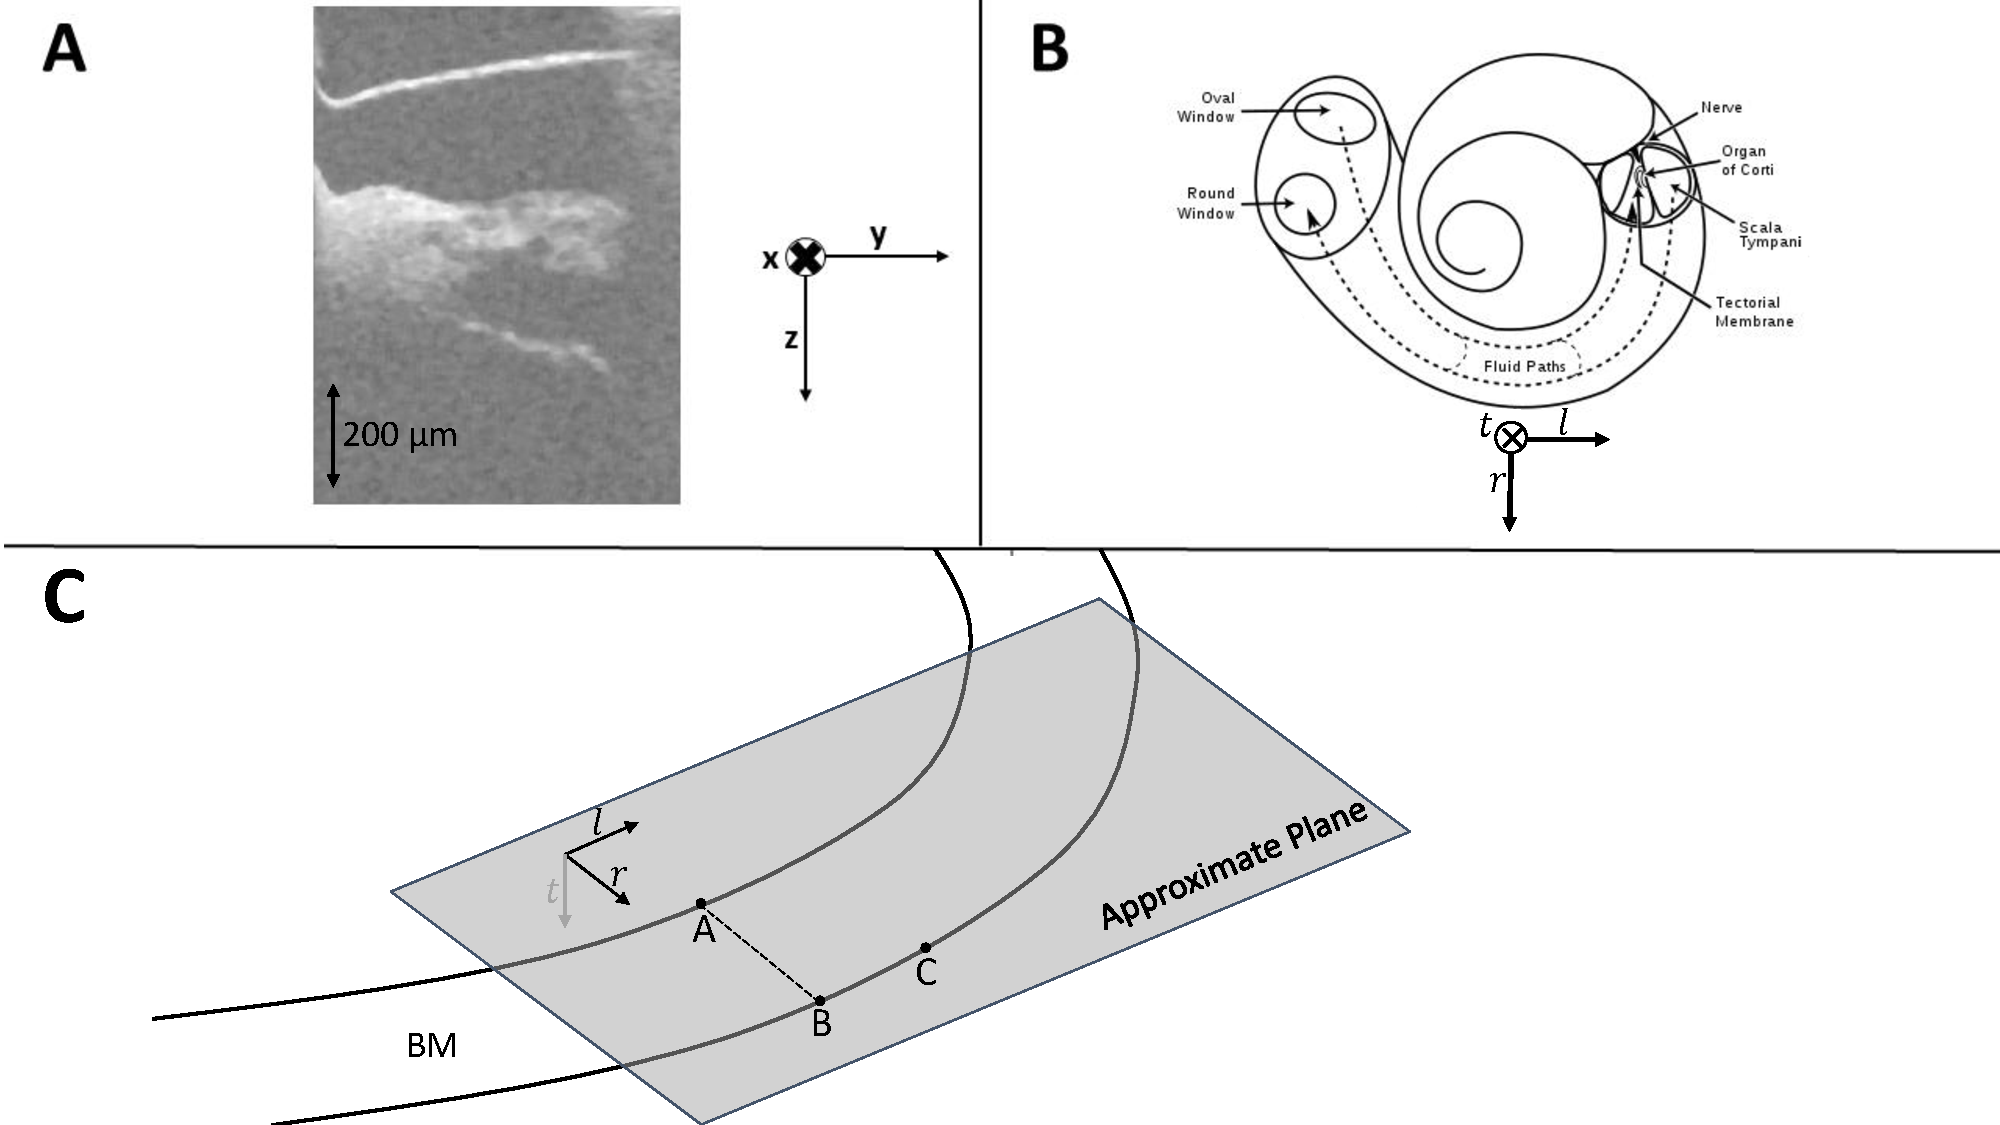
\includegraphics[width=\textwidth]{Figure2.pdf}
\caption{The coordinate systems used in the development of this program. \textbf{A} -- the optical coordinate system, defined with respect to the orienting B-Scan, shown alongside a representative B-Scan; \textbf{B} -- the anatomical coordinate frame, which varies so as to always be tangent to the BM at any point, shown at a point along a cartoon of the cochlea; \textbf{C} -- the local approximation of the anatomical coordinate system, defined with respect to a plane that approximates the BM's plane (shown as a gray surface).}
\label{coords}
\end{figure}

\subsection{Determining the Approximate Anatomical Plane}

\par{A volume scan is acquired using ThorImage software from Thorlabs, \textcolor{blue}{which allows the user to select the dimensions of the volume (which is always in the shape of a rectangular prism), as well as the spacing between the A-Scans which comprise the volume. In selecting the spacing, it is important to choose a spacing well below the lateral resolution of the OCT system so that as few as possible features are lost due to quantization. Our lateral resolution is about 10 $\mu$m, so we use 2 $\mu$m $\times$ 2 $\mu$m spacing. The axial spacing is determined by the bandwidth and wavelength of the light source, and is 2.7 $\mu$m \cite{OCTtheory}.} This volume is then imported into our coordinate transformation program. The volume scan is selected so that the orienting B-Scan lies in the center, where the volume comprises a set of  B-Scans parallel to this orienting B-Scan. As described above, at least two B-Scans are necessary to select points which define the local BM plane. So that the approximation is best near the orienting B-Scan, we choose two parallel B-Scans separated by $\Delta x$ in the $\mathbf{x}$ direction, equidistant from the orienting B-Scan. In the first of these B-Scans, we select two points on the BM,  $\mathbf{A}$ and $\mathbf{B}$. We select $\mathbf{B}$ to be the point on the BM nearest the outer wall and $\mathbf{A}$ to be the point nearest the spiral lamina. The BM in this cross-section should be well-approximated by the line segment $\overline{\mathbf{B}\mathbf{A}}$. \textcolor{blue}{(A video demonstrating these and subsequent steps is included as Supplemental Material.)}}
\par{We select the third point, $\mathbf{C}$, to be a point on the BM closest to the outer wall in the second B-Scan. We choose the second B-Scan to be apical to the orienting B-Scan (or mathematically, the projection of $\mathbf{l}$ onto $\overline{\mathbf{BC}}$ is positive).  As these three points determine the plane, we know the plane's unit normal vector \begin{equation}
\mathbf{t} = \frac{(\mathbf{A}-\mathbf{B})\times(\mathbf{C}-\mathbf{B})}{||(\mathbf{A}-\mathbf{B})\times(\mathbf{C}-\mathbf{B})||}.
\end{equation}
This vector $\mathbf{t}$ is the transverse unit vector -- the normal to the BM. We go on to find the longitudinal and radial vectors, $\mathbf{l}$ and $\mathbf{r}$. We selected both $\mathbf{B}$ and $\mathbf{C}$ to be points on the BM nearest to the outer wall, so that they lie at the same transverse and radial positions in two different anatomical cross-sections. Thereby, the vector 
\begin{equation}
\mathbf{l} = \frac{\mathbf{C}-\mathbf{B}}{||\mathbf{C}-\mathbf{B}||}
\end{equation}
is the local approximation of the longitudinal direction. To complete the right-handed coordinate system, the radial direction is given by 
\begin{equation}
\mathbf{r} = \mathbf{t}\times\mathbf{l}.
\end{equation}}


\par{Following this analysis, the anatomical coordinate vectors,  $\mathbf{r}, \mathbf{t}, \mathbf{l}$ are represented in the ordered basis of optical coordinates $\{\mathbf{x},\mathbf{y},\mathbf{z}\}$.  The $\mathbf{z}$ components of the anatomical coordinate vectors, $l_z$, $r_z$, and $t_z$, give the $\mathbf{z}$-axis (optical axis -- the direction of measurement), written in anatomical coordinates, and their relative sizes indicate the degree to which a given anatomical direction is represented in a measurement.}

\subsection{Determining the Coordinate Transformation}
\par{To proceed, our goal is to find the relationship between optical and anatomical coordinates. Now that we have represented the anatomical coordinates in a system that is stationary with respect to optical coordinates, this can be framed as a change of basis problem. A mapping between two coordinate systems is described by a unique change of basis matrix $U$. The process described above produces the anatomical coordinate vectors $\{\mathbf{l},\mathbf{r},\mathbf{t}\}$ in terms of optical coordinates. The mapping \textit{from anatomical to optical coordinates} is the $3\times 3$ matrix whose columns are the anatomical coordinate vectors written in optical coordinates, i.e.
\renewcommand*{\arraystretch}{.5}
\begin{equation}
U = \begin{pmatrix} l_{x} & r_{x} & t_{x} \\
l_{y} & r_{y} & t_{y} \\
l_{z} & r_{z} & t_{z}\end{pmatrix}.
\end{equation}}
\par{To explore the volume in anatomical coordinates, we map \textit{from optical to anatomical coordinates}. This is the inverse mapping of $U$. As all change of basis matrices are unitary, $U^{-1} = U^\text{T}$ maps from optical to anatomical coordinates.}


\subsection{Determining the Displacement Measurement Direction}
\par{Our first goal is to determine the direction of the vibratory motion we are measuring in anatomical coordinates. We refer to the displacement measurements along the optical ($\mathbf{z}$) axis as $d(\mathbf{p},f)$. This is a scalar-valued function of the position $\mathbf{p}$ and the frequency of the stimulus $f$. $d(\mathbf{p},f)$ is the $\mathbf{z}$ projection of the three-dimensional displacement $\mathbf{D}(\mathbf{p},f)$. We can write $\mathbf{D}(\mathbf{p},f)$ in the space of anatomical coordinates as follows:
\begin{equation}
\mathbf{D}(\mathbf{p},f) = D_l(\mathbf{p},f)\mathbf{l} + D_r(\mathbf{p},f)\mathbf{r} + D_t(\mathbf{p},f)\mathbf{t}.
\end{equation}}
\par{As we have expressed the unit vectors $\mathbf{l}$, $\mathbf{r}$ and $\mathbf{t}$ in the optical coordinates above, we know the $\mathbf{z}$-components of these unit vectors, which we write as $l_z$, $r_z$ and $t_z$ respectively. As such, our measurement is given by: \begin{equation}d(\mathbf{p},f) = D_l(\mathbf{p},f)l_z + D_r(\mathbf{p},f)r_z + D_t(\mathbf{p},f)t_z.
\end{equation}}
\par{In practice $l_z$, $r_z$ and $t_z$ are often all \textcolor{blue}{non-negligible}, and with a unidirectional motion measurement, we cannot determine $D_l$, $D_r$ and $D_t$ separately. (For clarity, consider the alternative -- if we were able to choose the optical axis to be perpendicular to the local plane of the BM, $l_z$ and $r_z$ would be zero, and $t_z$ would equal 1, so $d(\mathbf{p},f) =  D_t(\mathbf{p},f).)$}
\subsection{Exploring Optical Space in Anatomical Coordinates}

\par{The change of basis matrix $U$ gives us a simple way to explore the volume scan in terms of optical and anatomical coordinates simultaneously. We have developed a GUI, based in MATLAB and available upon request, that allows the user to traverse the volume in either coordinate system, shown in Fig. \ref{gui}. We refer to the GUI program as the \textit{orienting GUI}. As the user moves about the volume in one coordinate system, the other set of coordinates is computed by applying either $U$ or $U^T$ for anatomical-to-optical and optical-to-anatomical transformations respectively.  The red line represents the projection of the plane onto the B-Scan. Users can use sliders or enter values to traverse the volume in either coordinate system, and see the corresponding coordinates in both systems (anatomical on the left, optical on the right).} 

\begin{figure}[h!]
\centering
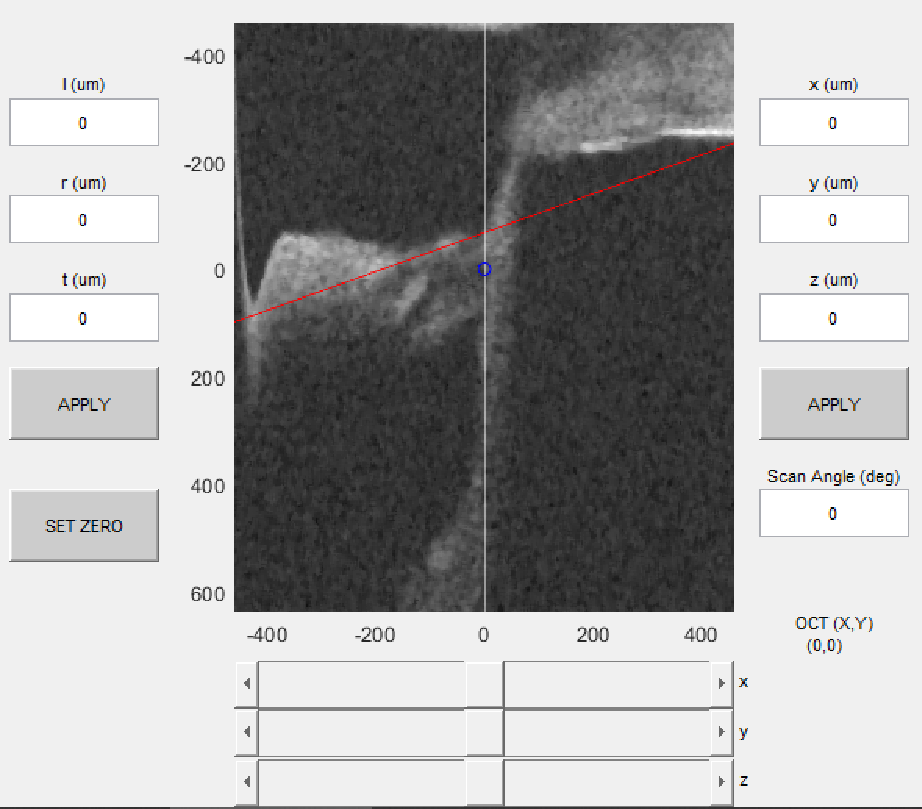
\includegraphics[width=0.7\textwidth]{Figure3.pdf}
\caption{GUI used to explore volumes in both optical and anatomical coordinates. Shown is the orienting B-Scan from experiment 900. The coordinate values of the blue point's location are shown in the anatomical (left) and optical (right) systems, and the A-Scan in which this point lies is shown in white. The red line is the planar approximation of the BM projected onto the displayed B-Scan.}
\label{gui}
\end{figure}

\par{The orienting GUI has two main purposes: 1) to find the anatomical locations of structures measured in one A-Scan, and 2) to pick locations for measurement (in optical coordinates) based on their anatomical locations. One important application is to measure vibrations of different structures (such as the BM and OHC) within the same anatomical cross-section (that is, same $\mathbf{l}$-coordinate value). This is achieved as follows: first observe an A-Scan in which both the BM and OHC are present. Then, use the orienting GUI to determine the longitudinal location of the OHCs relative to the BM in that A-Scan. Next, determine the optical coordinates of a position on the BM in the same anatomical cross-section as those OHCs.  Finally, use the OCT positioning mirrors to set the optical axis along each of these A-scans sequentially, and take motion measurements at each. This allows the measurement of the motion of OHCs and BM within the same anatomical cross-section.}
\par{\textcolor{blue}{It is important to note that structures within the OCC have tilts in longitudinal directions, so that measuring a part of a cell in the same longitudinal cross-section as the BM does not mean the \textit{entire} cell lies in the same longitudinal cross-section. However, the tilt of gerbil OHCs in the longitudinal direction is small (about $5^\text{o}$), so anatomical tilt has no significant effect on the application explored in the present work \cite{yoon}. Other structures in the OCC (in particular the Deiters cells' processes) have a significant longitudinal tilt that should be accounted for when their motion is measured.}}

\subsection{\textcolor{blue}{Sensitivity to Point Selection}}
\par{\textcolor{blue}{We close the Methods section by considering the sensitivity of our model to the choice of points $\mathbf{A}$, $\mathbf{B}$ and $\mathbf{C}$, in order to understand how variation in user input will affect the operation of our program. To explore this problem, we consider a particular volume scan from Experiment 903, and a corresponding planar approximation based on experimenter-selected points $\mathbf{A}$, $\mathbf{B}$ and $\mathbf{C}$. In determining these points, we used a 20 $\mu$m spacing between B-Scans. We consider the case in which two of these points are fixed and the third is selected at some point within a 40 $\mu$m $\times$ 40 $\mu$m square of the originally selected point (Fig. \ref{error} A and C). To contextualize this square, the lateral resolution of our OCT device is around 10 $\mu$m, and axial resolution is about 8 $\mu$m. That means that the square of tested values is about 4 $\times$ 5 units of optical resolution. Then, we consider the transverse unit vector computed by using this newly selected point, and compute the angle it makes with the original unit transverse vector, via the cosine rule of dot products. We do this %for $10^4$ points in this square
varying point $\mathbf{A}$ with $\mathbf{B}$ and $\mathbf{C}$ fixed, and again varying point $\mathbf{C}$ with $\mathbf{A}$ and $\mathbf{B}$ fixed. The two tested squares of points are shown in Fig. \ref{error} A and C. Fig. \ref{error} B and D show the results: the resulting variation in the angle of the transverse unit vector relative to the originally computed angle.}}
\par{\textcolor{blue}{The planar approximation is more sensitive to choice in the point $\mathbf{C}$ than point $\mathbf{A}$. This is unsurprising, as point $\mathbf{A}$ is far from both points $\mathbf{B}$ and $\mathbf{C}$, while point $\mathbf{C}$ is quite close to $\mathbf{B}$. The largest variation is about $15^\text{o}$, with point $\mathbf{C}$ chosen at the very edge of the test box, two units of lateral resolution and two and a half units of axial resolution away from the originally selected point. Next we explore the effect of this angular variation in the application of our program described above and performed in the Representative Example section below -- that is, the use of the program to locate OHCs and BM in the same longitudinal cross-section. For this application, we start with a point at the OHCs and then move purely in the computed transverse direction until we reach the BM. This distance is usually about 45 $\mu$m. %The computed points ``on the BM in the same longitudinal cross-section" are found by moving approximately 45 $\mu$m along these vectors. 
The angular variation from above, $\theta$, gives rise to a variation in distance that is calculated using the law of cosines:
\begin{equation}
    d_{BM} = 45\sqrt{2-2\cos\theta}.
\end{equation}
The distance variation computed from the angular variation is shown as a second color bar in Fig. \ref{error} B and D. (Note that this calculation corresponds to a displacement vector containing components in all three anatomical directions, and thus is an upper bound on the variation in the longitudinal distance, which is the variation important for our particular application.) A worst case distance variation of 12 $\mu$m is in the far upper-right of panel D. Within the more reasonable selection range of 20 $\mu$m $\times$ 20 $\mu$m about the selected point, we see a maximum variation of about 5 $\mu$m. This variation can be compared with the $\sim$ 40  $\mu$m longitudinal distance between OHCs and the BM within a single B-scan noted in the introduction.  Using 5 $\mu$m as the maximum variability with reasonably careful point selection, the use of the program to locate OHCs and BM in the same longitudinal cross-section will be accurate to $\sim$ 12\%.}} %the program will identify the and the traveling wave phase would vary by about 6 degrees \cite{Ren2002}. This example, which is representative of results found for other volumes, shows that our method is not critically sensitive to choice in these points.}}

\begin{figure}[h!]
\centering
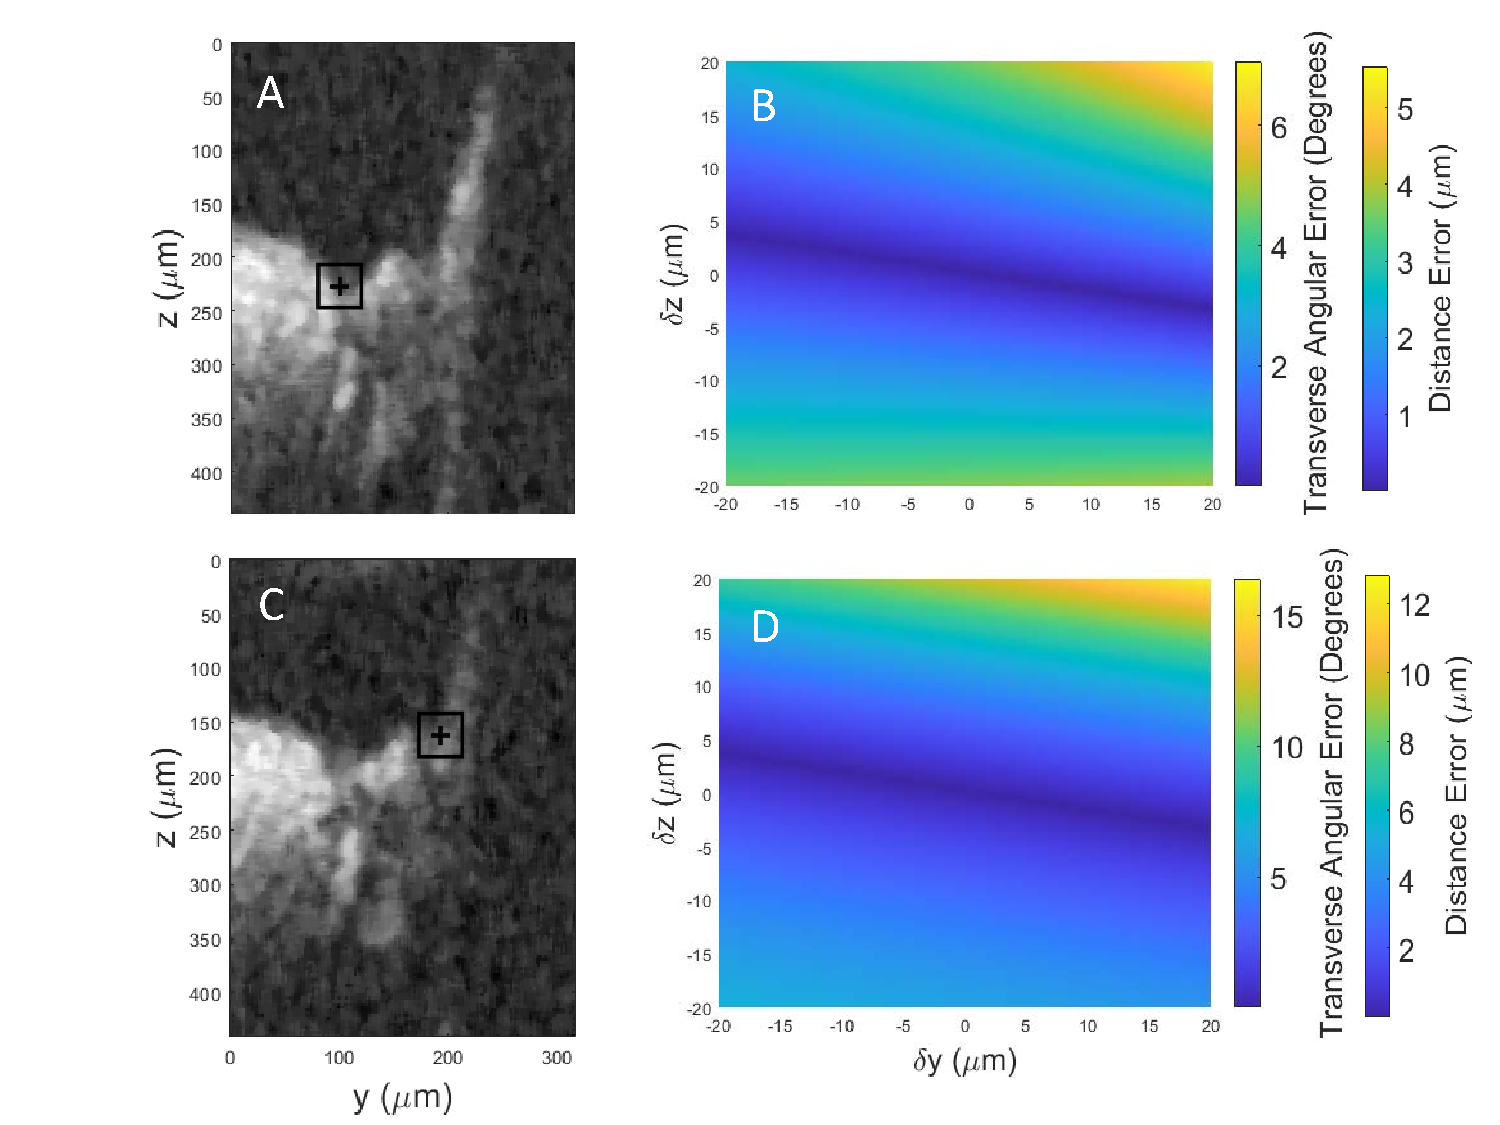
\includegraphics[width=\textwidth]{Figure4.pdf}
\caption{\textcolor{blue}{\textbf{A} -- A zoomed in B-Scan of the OCC in gerbil experiment 903, wherein points $\mathbf{A}$ and $\mathbf{B}$ are chosen. The experimenter's guess for point $\mathbf{A}$ is marked as a black cross, and the 40 $\mu$m $\times$ 40 $\mu$m box of tested $\mathbf{A}$ values is shown centered about this point. $\textbf{B}$ -- Angular difference between transverse unit vectors computed using the experimenter-chosen points and points in the box shown in panel A with points $\mathbf{B}$ and $\mathbf{C}$ fixed. The corresponding distance between computed BM positions is shown in a separate color bar to the right. \textbf{C} -- Similar to panel A, but in the second B-Scan in which $\mathbf{C}$ is chosen with the tested values of $\mathbf{C}$ shown. %Here, the second B-Scan was chosen to be 20 $\mu$m from the first in the optical $x$ direction. 
\textbf{D} -- Similar to panel B, but using different values of $\mathbf{C}$ and fixing points $\mathbf{A}$ and $\mathbf{B}$.}}
\label{error}
\end{figure}

\section{Results}

\subsection{Representative Example}

\par{We began with a 1 mm$\times$1 mm$\times$1.38 mm volume scan from gerbil through the round window. All data were taken using the ThorLabs Telesto 311 spectral domain OCT system using the LSM-03 objective lens. We used B-Scans $\Delta x = 20$ $\mu$m apart (each 10 $\mu$m from the orienting B-Scan) to choose points $\mathbf{A}$, $\mathbf{B}$ and $\mathbf{C}$, as shown in Fig. \ref{lines}. With these three points, we determined the anatomical coordinates $\mathbf{l}$, $\mathbf{r}$ and $\mathbf{t}$. This also allows us to find the displacement measurement breakdown: $d(\mathbf{p},f) = D_l(\mathbf{p},f)l_z + D_r(\mathbf{p},f)r_z + D_t(\mathbf{p},f)t_z.$ The uniaxial measurement does not allow us to determine $D_l, D_r$ and $D_t$ but it shows which of these anatomical motions our uniaxial measurement is most sensitive to. In our example, with a commonly used angle of approach through the round window, the component multipliers had values $l_z = 0.8$, $r_z = -0.1$ and $t_z = 0.6$. This shows that in this example the most represented anatomical component of motion was longitudinal, with significant representation in the transverse direction. $r_z$ was relatively small, meaning that the optical axis is nearly perpendicular to the radial axis, and thus a motion measurement along this optical axis is not very sensitive to radial vibration.}

\begin{figure}[h!]
\centering
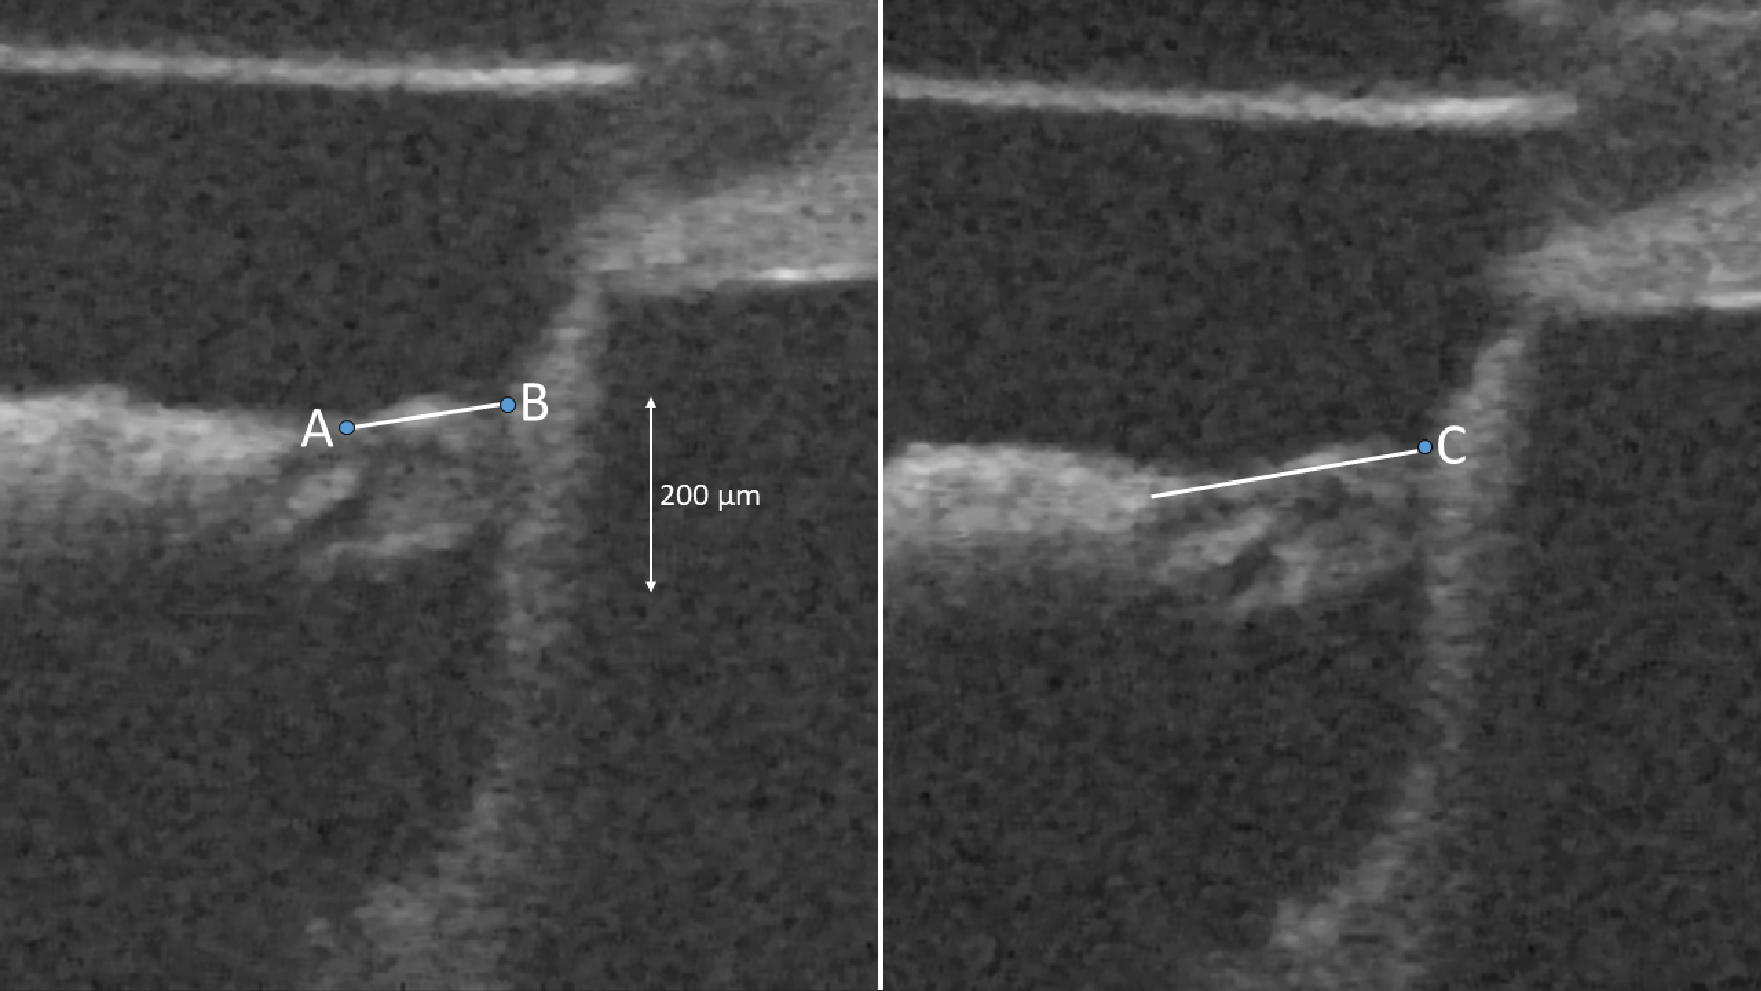
\includegraphics[width=\textwidth]{Figure5.pdf}
\caption{Plane approximation process, experiment 900. Two B-Scans from a single volume scan, 20 $\mu$m apart. Points $\mathbf{A}$ and $\mathbf{B}$ are chosen in the first B-Scan (left). This determines the line segment (shown in white) that approximates the BM in this cross-section. In the second B-Scan (right), $\mathbf{C}$ is chosen, completely defining the plane. The projection of that plane onto the second B-Scan is shown in white.}
\label{lines}
\end{figure}

\par{Next, we use the orienting GUI to find the anatomical positions of the BM and OHC region along the initial A-Scan, as shown in Fig. \ref{process} A and B.  We found that the OHCs in the initial A-scan lay about 45 $\mu$m apical from the BM. We then used the program to determine the optical coordinates of the BM 45 $\mu$m apical of the initial A-scan -- this is a point on the BM in the same anatomical cross-section as the OHCs in the initial A-Scan (Fig. \ref{process} C). We took vibration measurements along these two A-scans in two sequential data runs, using the quantitative output of the orienting GUI to position the OCT mirrors to access each A-Scan in turn. This process can also be seen in the video included as Supplemental Material.}

\begin{figure}[h!]
    \centering
    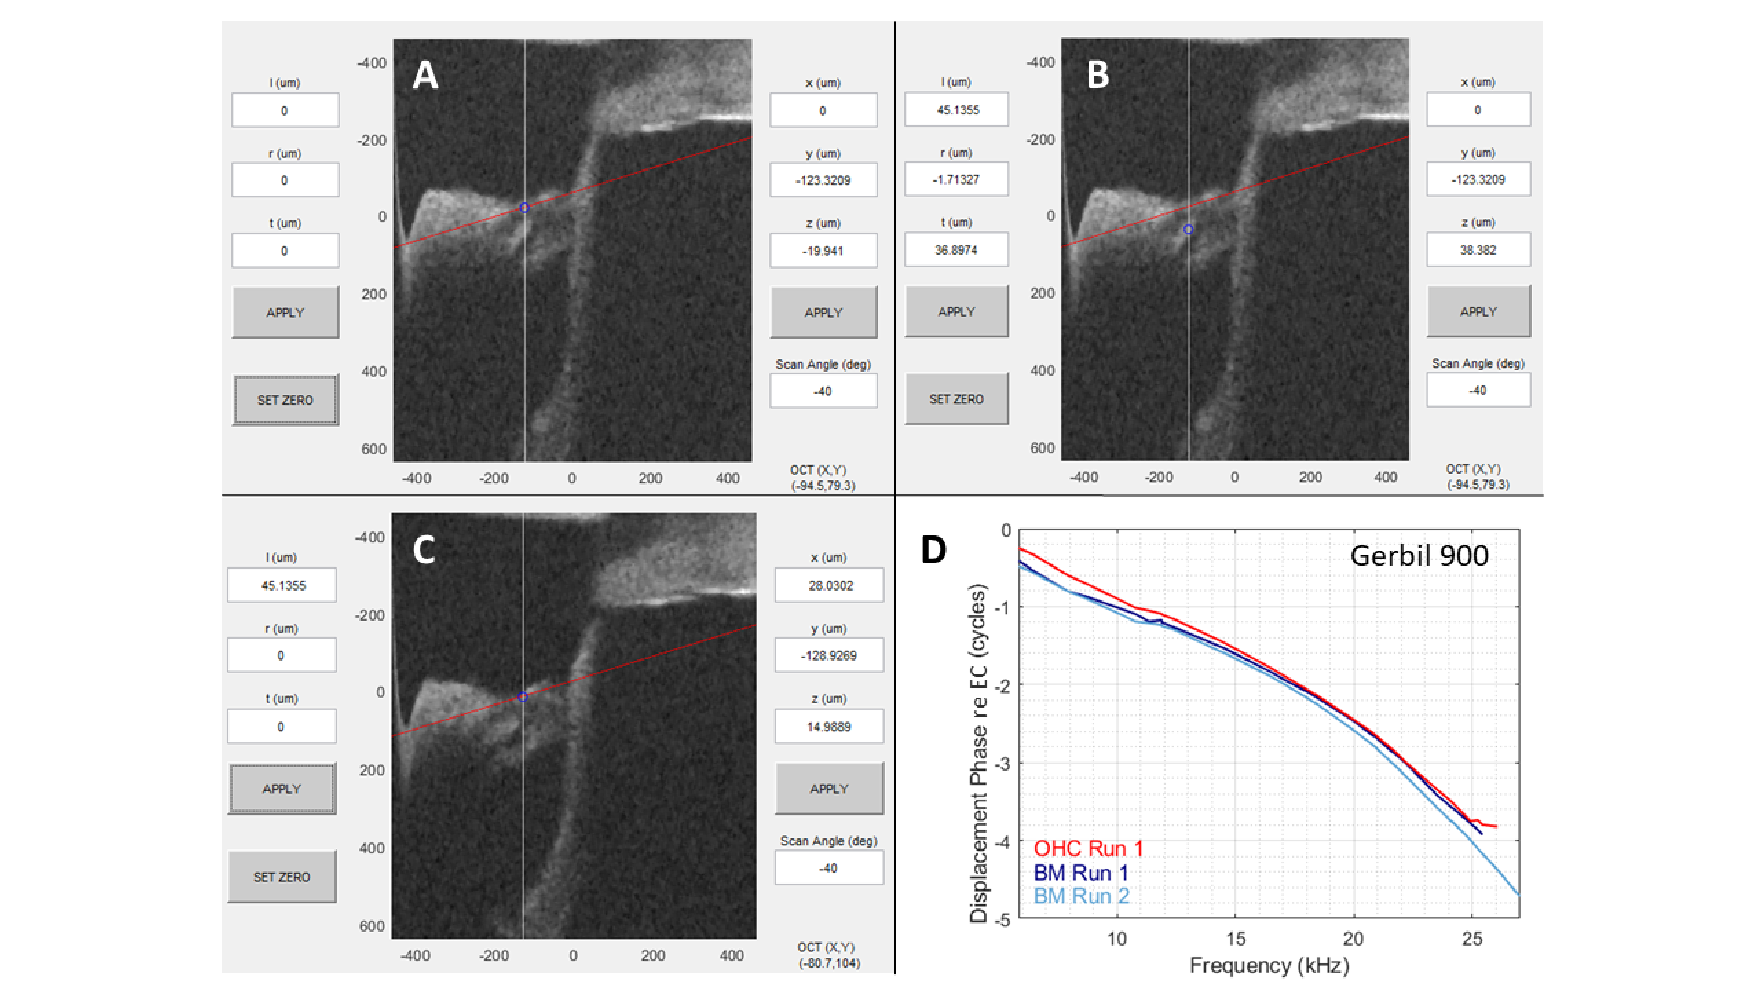
\includegraphics[width=\textwidth]{Figure6.pdf}
    \caption{Use of the orienting GUI to measure BM and OHC in the same anatomical cross-section. \textbf{A} -- To begin, we select an A-Scan containing BM and OHC. The zero point is set to be on the BM along this A-Scan, as shown here. \textbf{B} -- We move the $z$ slider so that the blue point is on the OHCs and the A-Scan has not changed. Only the $z$ optical coordinate changes, whereas all three anatomical coordinates have changed. The $l$ value indicates that the OHCs are about 45 $\mu$m apical of the BM in this A-Scan. \textbf{C} -- We find the measurement location necessary to measure BM motion in the same cross-section as OHC from the previous A-Scan by moving to the point with the same $l$ position but with $r=t=0$. The OCT(x,y) coordinates on the bottom right are the output data we use to direct the OCT positioning mirrors to the desired A-scan location.  \textbf{D} -- We display the measured displacement phase with respect to ear canal (EC) at the OHC and BM in the first A-Scan, as well as the BM in the second A-Scan. The OHC from run 1 and BM from run 2 are in the same anatomical cross-section.  Data taken at 80 dB SPL.}
    \label{process}
\end{figure}

\par{Panel D in Fig. \ref{process} shows the vibration phases of the BM and OHC-region from two A-Scan locations in the same animal --  Run 1 OHC and BM are in the same A-Scan, whereas Run 2 BM is in the same anatomical cross-section as run 1 OHC. The BM and OHC vibration phases can be compared as measured along one A-scan (red compared to dark blue) or as measured within a single anatomical cross-section (red compared to light blue). Comparing within an A-Scan, the OHC vibration phase led the BM significantly at low frequencies, with the lead diminishing to zero as frequency increased. On the other hand, comparing within the anatomical cross-section, OHC vibration led the BM over the entire frequency range. The difference in the BM vibration measurements in the two runs likely occurs due to the longitudinal progression of the phase of the cochlea's travelling wave, which is frequency dependent. In these results, the OHC-BM phase differences within one A-Scan deviated from the OHC-BM phase differences within an anatomical cross-section by as much as a quarter-cycle. In the analysis of cochlear mechanics, a quarter cycle phase ``error" could shift an interpretation of results from power-neutral to power-generating or power-absorbing.  Thus, this magnitude of potential phase-reporting-error significantly impacts the study of the operation of the cochlea and the cochlear amplifier \citep{cooper, dongolson, fallah}.}

\subsection{\textcolor{blue}{Testing Against} Known Physiology}
\par{To \textcolor{blue}{test the functionality of our method}, we used data from an \textit{in vivo} gerbil experiment in which our program was used to probe an established property of cochlear mechanics. It is known that at a given longitudinal position (anatomical cross-section), the phase of BM motion is approximately the same at all locations spanning the BM radially \citep{cooperMOHJapan, Warren}. We used the BM planar approximation and coordinate transformation (the orienting GUI) to take BM motion recordings at what we computed to be locations that were all at the same longitudinal position, at locations that spanned the BM radially. We performed this process within two volume scans, each taken at a different orientation of the gerbil's head with respect to the scanner. The volume scans were taken such that a single B-Scan was not perpendicular to the longitudinal axis, and thus orienting across the BM radially involved navigating through a series of B-Scans. Fig. \ref{radial} illustrates the concept, with the box region indicating the x-y plane of the volume scan. In the results shown in Fig. \ref{raddata}, the vibration phase did not change as the measurement location moved radially across the BM. Thus, our results confirmed established findings, indicating that the orienting GUI successfully identified the anatomical cross-section.} 

\begin{figure}[h!]
    \centering
    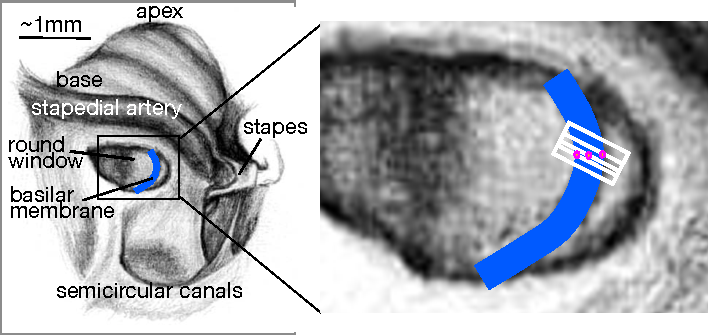
\includegraphics[width=0.7\textwidth]{Figure7.pdf}
    \caption{Illustration of the method used to \textcolor{blue}{test} the operation of the orienting GUI \textcolor{blue}{against known physiology}. The blue band in each view indicates the basilar membrane. The magenta dots in the expanded view on the right indicate points that span the BM radially. The white box is the $\mathbf{x}$-$\mathbf{y}$ plane of a volume scan, with the interior white lines indicating the $\mathbf{y}$ axis of the B-Scans in which the magenta points lie. The orienting GUI identifies the locations of the magenta points, all of which lie in different B-Scans.}
    \label{radial}
\end{figure}

\begin{figure}[h!]
    \centering
   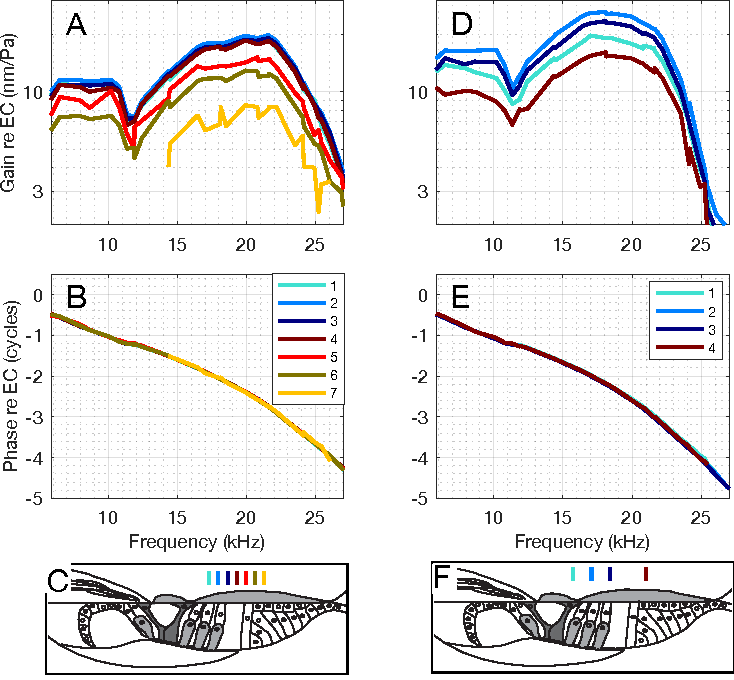
\includegraphics[width=\textwidth]{Figure8.pdf}
    \caption{BM displacement data from experiment 900 from two different head angles \textcolor{blue}{provide evidence} that the GUI orientation program correctly identified the anatomical radial axis. \textbf{A} and \textbf{B} -- BM displacement amplitude and phase taken along a single anatomical cross-section at seven radial locations spaced 10 $\mu$m apart medial (aqua) to lateral (yellow), \textcolor{blue}{with locations approximated in \textbf{C}}; \textbf{D} and \textbf{E} -- BM displacement amplitude and phase taken in a different anatomical cross-section at radial locations spaced 20 or 40 $\mu$m apart medial (aqua) to lateral (brown), \textcolor{blue}{with locations approximated in \textbf{F}}. Data taken at 80 dB SPL.}
    \label{raddata}
\end{figure}

\section{Conclusions}
\par{We have presented a method for determining the location and orientation of the structures in OCT volume scans relative to their canonical anatomical coordinates. This method requires the presence of a locally planar structure, and the experimenter's selection of three points within two parallel B-Scans. It is a simple and fast process by which to add meaning to OCT measurements. In the context of cochlear mechanics, this allows us to determine the components of motion that are represented in our vibration measurements. It also allows us to measure structures with certain anatomical relationships to one another, such as being in the same anatomical cross-section, despite their not lying in the same B-Scan. Being able to take measurements of different structures at the same anatomical cross-section allows for more direct motion comparisons to be made. We have shown that this corrects for travelling wave phase differences between structures in a single A-Scan. The method can be used to probe phase differences between OHCs, Hensen's cells, and the BM, furthering the detailed mapping of micromechanical motions and the understanding of cochlear operation.}
\par{While three-dimensional motion of the OCC can never be determined through a one-dimensional measurement, this program nevertheless offers insight into the results of three-dimensional cochlear models. When it is known which axis measurements are taken along, model results along this same axis can be compared to OCT measurements. In future work, measurements of the same structure taken at two or three known angles could be used to reconstruct two or three-dimensional motion.}

\clearpage
\bibliography{mybib.bib}

\end{document}